\documentclass[11pt,a4paper]{article}

% Packages
\usepackage[utf8]{inputenc}
\usepackage[T1]{fontenc}
\usepackage{amsmath,amssymb,amsthm}
\usepackage{graphicx}
\usepackage{hyperref}
\usepackage{listings}
\usepackage{xcolor}
\usepackage{geometry}
\usepackage{booktabs}
\usepackage{algorithm}
\usepackage{algpseudocode}
\usepackage{tikz}
\usetikzlibrary{arrows.meta,positioning,shapes.geometric}

% Page layout
\geometry{margin=1in}

% Code listing style
\definecolor{codegreen}{rgb}{0,0.6,0}
\definecolor{codegray}{rgb}{0.5,0.5,0.5}
\definecolor{codepurple}{rgb}{0.58,0,0.82}
\definecolor{backcolour}{rgb}{0.95,0.95,0.92}

\lstdefinestyle{pythonstyle}{
    backgroundcolor=\color{backcolour},
    commentstyle=\color{codegreen},
    keywordstyle=\color{magenta},
    numberstyle=\tiny\color{codegray},
    stringstyle=\color{codepurple},
    basicstyle=\ttfamily\footnotesize,
    breakatwhitespace=false,
    breaklines=true,
    captionpos=b,
    keepspaces=true,
    numbers=left,
    numbersep=5pt,
    showspaces=false,
    showstringspaces=false,
    showtabs=false,
    tabsize=2,
    language=Python
}

\lstset{style=pythonstyle}

% Theorem environments
\newtheorem{definition}{Definition}[section]
\newtheorem{theorem}{Theorem}[section]
\newtheorem{example}{Example}[section]

% Title
\title{\textbf{Structural Causal Models for Synthetic Data Generation\\in Uncertainty Quantification Systems}}
\author{AZIMUTH Project\\Uncertainty Predictor Module}
\date{\today}

\begin{document}

\maketitle

\begin{abstract}
This document provides comprehensive technical documentation for the Structural Causal Model (SCM) framework integrated into the AZIMUTH uncertainty quantification system. We present the mathematical foundations of SCMs, their implementation architecture, two concrete dataset examples (a generic parent-child model and a laser power physics-based model), and their integration with the uncertainty predictor training pipeline. This documentation serves both as a reference manual and as a guide for extending the system with custom causal models.
\end{abstract}

\tableofcontents
\clearpage

%=============================================================================
\section{Introduction}
%=============================================================================

\subsection{Motivation}

In uncertainty quantification for manufacturing and industrial processes, access to large, labeled datasets with known ground-truth relationships is often limited. The Structural Causal Model (SCM) framework addresses this challenge by enabling:

\begin{itemize}
    \item \textbf{Synthetic data generation} with controllable causal relationships
    \item \textbf{Rapid prototyping} without requiring real manufacturing data
    \item \textbf{Testing and validation} of uncertainty quantification algorithms
    \item \textbf{Physics-informed datasets} that encode domain knowledge
    \item \textbf{Reproducible experiments} with deterministic random seeds
\end{itemize}

\subsection{System Overview}

The SCM framework in AZIMUTH consists of three main components:

\begin{enumerate}
    \item \textbf{SCM Engine} (\texttt{scm\_ds/scm.py}): Core causal modeling framework
    \item \textbf{Dataset Definitions} (\texttt{scm\_ds/datasets.py}): Pre-configured causal models
    \item \textbf{Integration Layer} (\texttt{src/data/preprocessing.py}): Bridge to uncertainty predictor
\end{enumerate}

The system supports both synthetic SCM-generated data and real CSV data, with seamless switching via configuration files.

%=============================================================================
\section{Mathematical Foundations}
%=============================================================================

\subsection{Structural Causal Models}

\begin{definition}[Structural Causal Model]
A Structural Causal Model is a tuple $\mathcal{M} = (\mathbf{V}, \mathbf{U}, \mathcal{F})$ where:
\begin{itemize}
    \item $\mathbf{V} = \{V_1, \ldots, V_n\}$ is a set of endogenous (observed) variables
    \item $\mathbf{U} = \{U_1, \ldots, U_n\}$ is a set of exogenous (noise) variables
    \item $\mathcal{F} = \{f_1, \ldots, f_n\}$ is a set of structural functions where each $f_i$ defines:
    \[
    V_i = f_i(\text{Pa}(V_i), U_i)
    \]
    where $\text{Pa}(V_i) \subseteq \mathbf{V} \setminus \{V_i\}$ are the parents of $V_i$ in the causal graph.
\end{itemize}
\end{definition}

\subsection{DAG Constraint}

The structural equations must form a Directed Acyclic Graph (DAG):

\begin{theorem}[Acyclicity Requirement]
The parent-child relationships defined by $\mathcal{F}$ must induce a DAG, i.e., there exists a topological ordering $\pi: \mathbf{V} \to \{1, \ldots, n\}$ such that for all $V_i, V_j \in \mathbf{V}$:
\[
V_i \in \text{Pa}(V_j) \implies \pi(V_i) < \pi(V_j)
\]
\end{theorem}

This enables forward evaluation: variables can be computed sequentially following the topological order.

\subsection{Sampling from SCMs}

Given an SCM $\mathcal{M}$, we generate $N$ i.i.d. samples as follows:

\begin{algorithm}
\caption{SCM Sampling Algorithm}
\begin{algorithmic}[1]
\Require SCM $\mathcal{M} = (\mathbf{V}, \mathbf{U}, \mathcal{F})$, sample size $N$, random seed $s$
\Ensure DataFrame with $N$ rows and $|\mathbf{V}|$ columns
\State Initialize random generator: $\text{rng} \gets \text{default\_rng}(s)$
\State Compute topological order: $[V_{\pi(1)}, \ldots, V_{\pi(n)}] \gets \text{TopoSort}(\mathcal{F})$
\State Sample noise: $\{u_i^{(1)}, \ldots, u_i^{(N)}\} \sim \text{Noise}_i(\text{rng}, N)$ for all $i$
\State Initialize context: $\text{ctx} \gets \{\}$
\For{$k = 1$ to $n$}
    \State $V_i \gets V_{\pi(k)}$
    \State Retrieve parent values: $\text{args} \gets [\text{ctx}[\text{pa}] \mid \text{pa} \in \text{Pa}(V_i)]$
    \State Compute: $\text{ctx}[V_i] \gets f_i(\text{args}, u_i^{(1:N)})$ \Comment{Vectorized evaluation}
\EndFor
\State \Return DataFrame$(\text{ctx})$
\end{algorithmic}
\end{algorithm}

\subsection{Pearl's do-Operator}

The framework supports interventional queries via Pearl's $do$-operator:

\begin{definition}[Intervention]
An intervention $do(V_i = c)$ on variable $V_i$ creates a mutilated SCM $\mathcal{M}_{V_i=c}$ where:
\[
f_i(\text{Pa}(V_i), U_i) \text{ is replaced by } f_i^* = c
\]
All other structural equations remain unchanged.
\end{definition}

This enables causal inference and counterfactual reasoning on the generated datasets.

%=============================================================================
\section{Implementation Architecture}
%=============================================================================

\subsection{Core Classes}

\subsubsection{NodeSpec}

The \texttt{NodeSpec} class defines a single node in the causal graph:

\begin{lstlisting}[caption={NodeSpec Structure}]
@dataclass(frozen=True)
class NodeSpec:
    name: str              # Unique node identifier
    parents: List[str]     # Parent node names (ordered)
    expr: str              # SymPy-compatible expression
\end{lstlisting}

\textbf{Example:}
\begin{lstlisting}
NodeSpec("Y", ["X", "Z"], "2*X + 0.5*Z + eps_Y")
\end{lstlisting}
defines $Y = 2X + 0.5Z + \varepsilon_Y$ where $\varepsilon_Y$ is the noise term.

\subsubsection{NoiseModel}

The \texttt{NoiseModel} class orchestrates noise generation:

\begin{lstlisting}[caption={NoiseModel Interface}]
class NoiseModel:
    def __init__(
        self,
        singles: Dict[str, NoiseSampler],  # Independent noises
        groups: List[GroupNoise]            # Correlated noises (MVN)
    ):
        ...

    def sample_all(self, rng, n) -> Dict[str, np.ndarray]:
        # Returns noise arrays for all nodes
\end{lstlisting}

\textbf{Noise sampler signature:}
\begin{lstlisting}
NoiseSampler = Callable[[np.random.Generator, int], np.ndarray]
\end{lstlisting}

For correlated noise (e.g., latent confounders), use \texttt{GroupNoise}:
\begin{lstlisting}
GroupNoise(
    nodes=("Z", "Y"),
    sampler=lambda rng, n: rng.multivariate_normal(
        mean=[0, 0],
        cov=[[1.0, 0.3], [0.3, 1.0]],
        size=n
    )
)
\end{lstlisting}

\subsubsection{SCM Class}

The \texttt{SCM} class is the execution engine:

\begin{lstlisting}[caption={SCM Core Methods}]
class SCM:
    def __init__(
        self,
        specs: Sequence[NodeSpec],
        noise_model: NoiseModel,
        backend: str = "numpy"
    ):
        # Validates DAG, compiles expressions via SymPy

    def sample(self, n: int, seed: int = 0) -> pd.DataFrame:
        # Generates n observational samples

    def do(self, interventions: Dict[str, float]) -> SCM:
        # Returns intervened SCM (do-operator)

    def adjacency(self, ...) -> pd.DataFrame:
        # Returns adjacency matrix
\end{lstlisting}

\textbf{Key implementation details:}
\begin{itemize}
    \item Expressions are compiled to NumPy functions via SymPy's \texttt{lambdify}
    \item Topological sort ensures correct evaluation order (Kahn's algorithm)
    \item Vectorized operations enable efficient batch generation
\end{itemize}

\subsubsection{SCMDataset Class}

The \texttt{SCMDataset} class wraps an SCM for machine learning tasks:

\begin{lstlisting}[caption={SCMDataset Interface}]
class SCMDataset:
    def __init__(
        self,
        name: str,
        description: str,
        specs: List[NodeSpec],
        singles: Dict[str, NoiseSampler],
        groups: List[GroupNoise],
        input_labels: List[str],   # Features for ML
        target_labels: List[str],  # Targets for ML
        ...
    ):
        self.scm = ...  # Compiled SCM
        self.input_labels = input_labels
        self.target_labels = target_labels

    def sample(self, n: int, seed: int = 42) -> pd.DataFrame:
        # Returns full DataFrame with all nodes
\end{lstlisting}

%=============================================================================
\section{Dataset Implementations}
%=============================================================================

\subsection{Dataset 1: Parent-Child with Cross-Talk}

\subsubsection{Causal Structure}

The \texttt{one\_to\_one\_ct} dataset models a system with 5 parent-child pairs and cross-talk:

\begin{center}
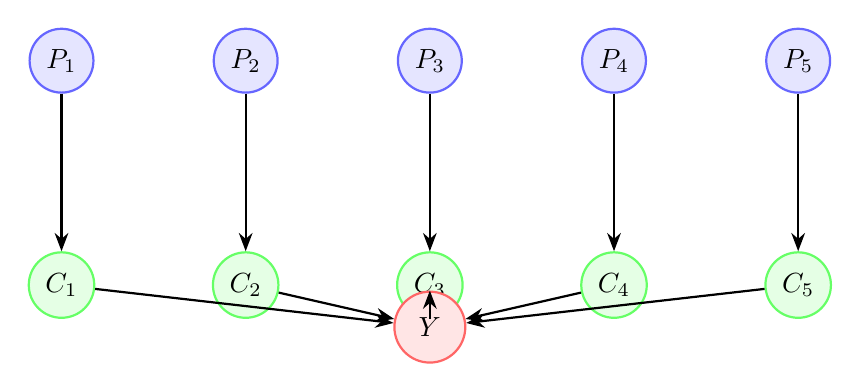
\begin{tikzpicture}[
    node distance=2cm and 1.5cm,
    parent/.style={circle, draw=blue!60, fill=blue!10, thick, minimum size=7mm},
    child/.style={circle, draw=green!60, fill=green!10, thick, minimum size=7mm},
    output/.style={circle, draw=red!60, fill=red!10, thick, minimum size=9mm},
    arrow/.style={-Stealth, thick}
]
    % Parents
    \node[parent] (P1) {$P_1$};
    \node[parent, right=of P1] (P2) {$P_2$};
    \node[parent, right=of P2] (P3) {$P_3$};
    \node[parent, right=of P3] (P4) {$P_4$};
    \node[parent, right=of P4] (P5) {$P_5$};

    % Children
    \node[child, below=of P1] (C1) {$C_1$};
    \node[child, below=of P2] (C2) {$C_2$};
    \node[child, below=of P3] (C3) {$C_3$};
    \node[child, below=of P4] (C4) {$C_4$};
    \node[child, below=of P5] (C5) {$C_5$};

    % Output
    \node[output, below=2.5cm of P3] (Y) {$Y$};

    % Arrows
    \draw[arrow] (P1) -- (C1);
    \draw[arrow] (P2) -- (C2);
    \draw[arrow] (P3) -- (C3);
    \draw[arrow] (P4) -- (C4);
    \draw[arrow] (P5) -- (C5);

    \draw[arrow] (C1) -- (Y);
    \draw[arrow] (C2) -- (Y);
    \draw[arrow] (C3) -- (Y);
    \draw[arrow] (C4) -- (Y);
    \draw[arrow] (C5) -- (Y);
\end{tikzpicture}
\end{center}

\subsubsection{Structural Equations}

\begin{align}
P_i &\sim \mathcal{N}(0, 1) \quad \text{for } i = 1, \ldots, 5 \\
C_i &= P_i + \varepsilon_{C_i}, \quad \varepsilon_{C_i} \sim \mathcal{N}(0, 1) \\
Y &= \sum_{i=1}^{5} C_i + \varepsilon_Y, \quad \varepsilon_Y \sim \mathcal{N}(0, 1)
\end{align}

\subsubsection{Implementation}

\begin{lstlisting}[caption={One-to-One Cross-Talk Dataset Definition}]
ds_scm_1_to_1_ct = SCMDataset(
    name="one-to-one_with_crosstalk",
    description="Every parent has one child with cross-talk",
    specs=[
        # Parents (exogenous)
        NodeSpec("P1", [], "eps_P1"),
        NodeSpec("P2", [], "eps_P2"),
        NodeSpec("P3", [], "eps_P3"),
        NodeSpec("P4", [], "eps_P4"),
        NodeSpec("P5", [], "eps_P5"),

        # Children (endogenous)
        NodeSpec("C1", ["P1"], "P1 + eps_C1"),
        NodeSpec("C2", ["P2"], "P2 + eps_C2"),
        NodeSpec("C3", ["P3"], "P3 + eps_C3"),
        NodeSpec("C4", ["P4"], "P4 + eps_C4"),
        NodeSpec("C5", ["P5"], "P5 + eps_C5"),

        # Output
        NodeSpec("Y", ["C1", "C2", "C3", "C4", "C5"],
                 "C1 + C2 + C3 + C4 + C5 + eps_Y"),
    ],
    singles={
        "P1": lambda rng, n: rng.standard_normal(n),
        "P2": lambda rng, n: rng.standard_normal(n),
        "P3": lambda rng, n: rng.standard_normal(n),
        "P4": lambda rng, n: rng.standard_normal(n),
        "P5": lambda rng, n: rng.standard_normal(n),
        "C1": lambda rng, n: rng.standard_normal(n),
        "C2": lambda rng, n: rng.standard_normal(n),
        "C3": lambda rng, n: rng.standard_normal(n),
        "C4": lambda rng, n: rng.standard_normal(n),
        "C5": lambda rng, n: rng.standard_normal(n),
        "Y":  lambda rng, n: rng.standard_normal(n),
    },
    input_labels=["P1", "P2", "P3", "P4", "P5",
                  "C1", "C2", "C3", "C4", "C5"],
    target_labels=["Y"]
)
\end{lstlisting}

\subsubsection{Properties}

\begin{itemize}
    \item \textbf{Input dimension:} 10 features
    \item \textbf{Output dimension:} 1 target
    \item \textbf{Noise model:} All independent Gaussian $\mathcal{N}(0,1)$
    \item \textbf{Use case:} Generic testing, baseline experiments
\end{itemize}

%-----------------------------------------------------------------------------
\subsection{Dataset 2: Laser Actual Power (Physics-Based)}

\subsubsection{Physical Motivation}

This dataset models laser output power as a function of target power setpoint and ambient temperature, incorporating the Light-Current-Temperature (L-I-T) relationship from semiconductor laser physics.

\subsubsection{Causal Structure}

\begin{center}
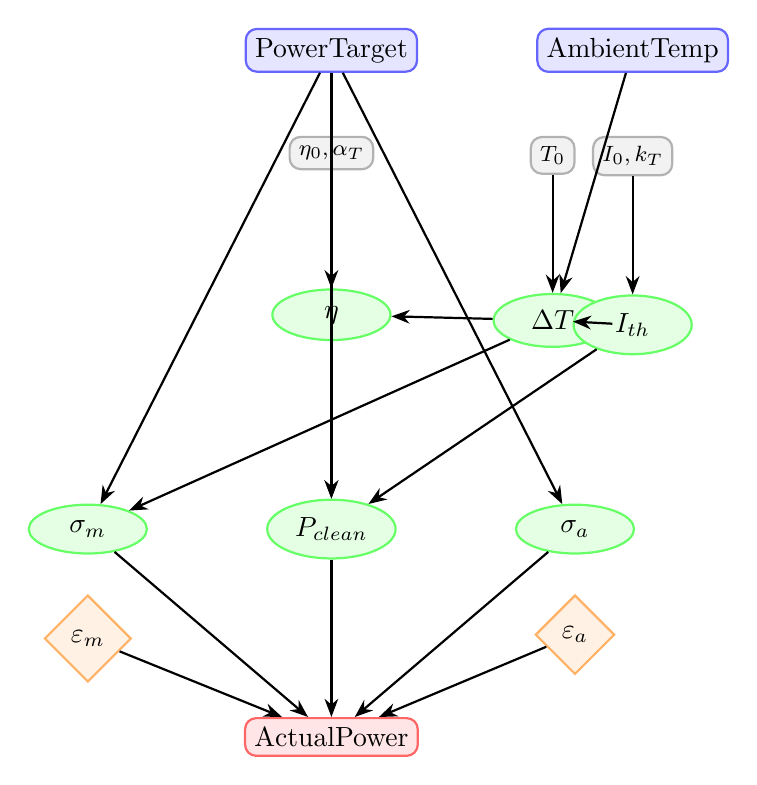
\begin{tikzpicture}[
    node distance=1.8cm and 1.2cm,
    input/.style={rectangle, draw=blue!60, fill=blue!10, thick, rounded corners},
    const/.style={rectangle, draw=gray!60, fill=gray!10, thick, rounded corners, font=\footnotesize},
    inter/.style={ellipse, draw=green!60, fill=green!10, thick, minimum width=1.5cm},
    noise/.style={diamond, draw=orange!60, fill=orange!10, thick, minimum size=7mm},
    output/.style={rectangle, draw=red!60, fill=red!10, thick, rounded corners, minimum width=1.5cm},
    arrow/.style={-Stealth, thick}
]
    % Row 1: Inputs
    \node[input] (I) {PowerTarget};
    \node[input, right=1.5cm of I] (T) {AmbientTemp};

    % Row 2: Constants (compact)
    \node[const, below left=0.8cm and -0.5cm of T] (T0) {$T_0$};
    \node[const, below=0.8cm of I] (eta) {$\eta_0, \alpha_T$};
    \node[const, below=0.8cm of T] (Ith) {$I_0, k_T$};

    % Row 3: Intermediates
    \node[inter, below=1.5cm of T0] (dT) {$\Delta T$};
    \node[inter, below=1.5cm of eta] (eff) {$\eta$};
    \node[inter, below=1.5cm of Ith] (Ithval) {$I_{th}$};

    % Row 4: Clean power
    \node[inter, below=2cm of eff] (Pclean) {$P_{clean}$};

    % Row 5: Noise scales
    \node[inter, left=1.5cm of Pclean] (sigM) {$\sigma_m$};
    \node[inter, right=1.5cm of Pclean] (sigA) {$\sigma_a$};

    % Noise sources
    \node[noise, below=0.5cm of sigM] (noiseM) {$\varepsilon_m$};
    \node[noise, below=0.5cm of sigA] (noiseA) {$\varepsilon_a$};

    % Output
    \node[output, below=2cm of Pclean] (P) {ActualPower};

    % Arrows
    \draw[arrow] (T) -- (dT);
    \draw[arrow] (T0) -- (dT);
    \draw[arrow] (eta) -- (eff);
    \draw[arrow] (dT) -- (eff);
    \draw[arrow] (Ith) -- (Ithval);
    \draw[arrow] (dT) -- (Ithval);
    \draw[arrow] (eff) -- (Pclean);
    \draw[arrow] (I) -- (Pclean);
    \draw[arrow] (Ithval) -- (Pclean);

    \draw[arrow] (dT) -- (sigM);
    \draw[arrow] (I) -- (sigM);
    \draw[arrow] (I) -- (sigA);

    \draw[arrow] (Pclean) -- (P);
    \draw[arrow] (sigM) -- (P);
    \draw[arrow] (sigA) -- (P);
    \draw[arrow] (noiseM) -- (P);
    \draw[arrow] (noiseA) -- (P);
\end{tikzpicture}
\end{center}

\subsubsection{Structural Equations}

\textbf{Inputs:}
\begin{align}
I &= \text{PowerTarget} \sim \mathcal{U}(0.05, 1.0) \\
T &= \text{AmbientTemp} \sim 25 + 3 \cdot \mathcal{U}(-6, +6) \quad \text{(°C)}
\end{align}

\textbf{Intermediates:}
\begin{align}
\Delta T &= T - T_0 \quad \text{where } T_0 = 25\,°\text{C} \\
I_{th} &= I_0 \exp(k_T \Delta T) \quad \text{(threshold current)} \\
\eta &= \eta_0 (1 - \alpha_T \Delta T) \quad \text{(efficiency)} \\
P_{clean} &= \eta (I - I_{th}) \quad \text{(ideal power)}
\end{align}

\textbf{Heteroscedastic noise scales:}
\begin{align}
\sigma_m(T, I) &= \sigma_{m0} + c_T |\Delta T| + c_I \frac{I}{I_{max}} \\
\sigma_a(I) &= \sigma_{a0} P_{FS} + d_I P_{FS} \frac{I}{I_{max}}
\end{align}

\textbf{Output with heteroscedastic noise:}
\begin{equation}
P_{actual} = P_{clean} (1 + \sigma_m \varepsilon_m) + \sigma_a \varepsilon_a
\end{equation}
where $\varepsilon_m, \varepsilon_a \sim \mathcal{N}(0, 1)$.

\subsubsection{Physical Parameters}

\begin{table}[h]
\centering
\begin{tabular}{@{}lll@{}}
\toprule
Parameter & Value & Physical Meaning \\
\midrule
$\eta_0$ & 1.0 & Nominal efficiency \\
$\alpha_T$ & 0.005 & Efficiency loss per °C \\
$I_0$ & 0.10 & Threshold current (normalized) \\
$k_T$ & 0.03 & Threshold growth per °C \\
$T_0$ & 25.0 °C & Reference temperature \\
$\sigma_{m0}$ & 0.01 & Base multiplicative noise \\
$c_T$ & 0.0005 & Temperature-dependent noise \\
$c_I$ & 0.01 & Current-dependent noise \\
$\sigma_{a0}$ & 0.005 & Base additive noise \\
$d_I$ & 0.002 & Current-dependent additive noise \\
\bottomrule
\end{tabular}
\caption{Laser SCM Physical Parameters}
\end{table}

\subsubsection{Implementation Notes}

\textbf{Key design pattern for constants in SCM:}

Constants (like $\eta_0$, $T_0$) are implemented as deterministic nodes:
\begin{lstlisting}
# Node definition:
NodeSpec("ETA0", [], "eps_ETA0")

# Noise sampler (returns constant):
"ETA0": lambda rng, n: np.full(n, 1.0)
\end{lstlisting}

This ensures compatibility with the SCM framework requirement that \emph{every node must have exactly one noise sampler}.

\textbf{Separate noise nodes:}

To handle heteroscedastic noise with two independent sources:
\begin{lstlisting}
NodeSpec("NoiseM", [], "eps_NoiseM")  # Multiplicative
NodeSpec("NoiseA", [], "eps_NoiseA")  # Additive

NodeSpec("ActualPower",
         ["Pclean", "SigmaM", "NoiseM", "SigmaA", "NoiseA"],
         "Pclean * (1 + SigmaM * NoiseM) + SigmaA * NoiseA + ...")
\end{lstlisting}

\subsubsection{Properties}

\begin{itemize}
    \item \textbf{Input dimension:} 2 features (PowerTarget, AmbientTemp)
    \item \textbf{Output dimension:} 1 target (ActualPower)
    \item \textbf{Noise model:} Heteroscedastic (state-dependent variance)
    \item \textbf{Use case:} Laser manufacturing, physics-informed ML
\end{itemize}

%=============================================================================
\section{Integration with Uncertainty Predictor}
%=============================================================================

\subsection{System Architecture}

\begin{center}
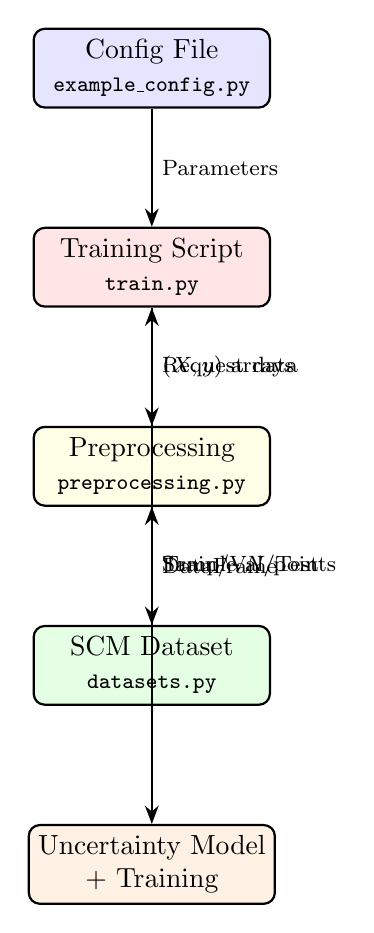
\begin{tikzpicture}[
    node distance=1.5cm,
    box/.style={rectangle, draw, rounded corners, thick, minimum width=3cm, minimum height=1cm, align=center},
    config/.style={box, fill=blue!10},
    scm/.style={box, fill=green!10},
    prep/.style={box, fill=yellow!10},
    train/.style={box, fill=red!10},
    arrow/.style={-Stealth, thick}
]
    \node[config] (config) {Config File\\{\footnotesize \texttt{example\_config.py}}};
    \node[train, below=of config] (train) {Training Script\\{\footnotesize \texttt{train.py}}};
    \node[prep, below=of train] (prep) {Preprocessing\\{\footnotesize \texttt{preprocessing.py}}};
    \node[scm, below=of prep] (scm) {SCM Dataset\\{\footnotesize \texttt{datasets.py}}};
    \node[box, below=of scm, fill=orange!10] (model) {Uncertainty Model\\+ Training};

    \draw[arrow] (config) -- node[right, font=\footnotesize] {Parameters} (train);
    \draw[arrow] (train) -- node[right, font=\footnotesize] {Request data} (prep);
    \draw[arrow] (prep) -- node[right, font=\footnotesize] {Sample $N$ points} (scm);
    \draw[arrow] (scm) -- node[right, font=\footnotesize] {DataFrame} (prep);
    \draw[arrow] (prep) -- node[right, font=\footnotesize] {$(X, y)$ arrays} (train);
    \draw[arrow] (train) -- node[right, font=\footnotesize] {Train/Val/Test} (model);
\end{tikzpicture}
\end{center}

\subsection{Configuration Layer}

The user specifies the data source in \texttt{configs/example\_config.py}:

\begin{lstlisting}[caption={Configuration Example}]
CONFIG = {
    'data': {
        # Option 1: Real data from CSV
        'csv_path': 'path/to/data.csv',
        'input_columns': ['x', 'y', 'z'],
        'output_columns': ['res_1'],

        # Option 2: SCM synthetic data
        'csv_path': None,  # Set to None to use SCM
        'use_scm': True,
        'scm': {
            'n_samples': 5000,
            'seed': 42,
            'dataset_type': 'one_to_one_ct'  # or 'laser'
        },

        # Common settings
        'scaling_method': 'standard',
        'train_size': 0.7,
        'val_size': 0.15,
        'test_size': 0.15,
    },
    # ... model, training configs
}
\end{lstlisting}

\subsection{Data Loading Logic}

The \texttt{train.py} script implements conditional data loading:

\begin{lstlisting}[caption={Data Source Selection in train.py}]
# Determine data source
csv_path = CONFIG['data'].get('csv_path')
use_scm = CONFIG['data'].get('use_scm', False)
use_csv = csv_path is not None and Path(csv_path).exists()

if use_csv:
    # Load from CSV
    X, y = load_csv_data(
        csv_path,
        CONFIG['data']['input_columns'],
        CONFIG['data']['output_columns']
    )
    input_columns = CONFIG['data']['input_columns']
    output_columns = CONFIG['data']['output_columns']

elif use_scm:
    # Generate synthetic data via SCM
    scm_config = CONFIG['data'].get('scm', {})
    X, y, input_columns, output_columns = generate_scm_data(
        n_samples=scm_config.get('n_samples', 5000),
        seed=scm_config.get('seed', 42),
        dataset_type=scm_config.get('dataset_type', 'one_to_one_ct')
    )
else:
    raise ValueError("No data source specified")
\end{lstlisting}

\subsection{SCM Data Generation Function}

The \texttt{generate\_scm\_data} function in \texttt{preprocessing.py} handles SCM instantiation:

\begin{lstlisting}[caption={SCM Data Generation}]
def generate_scm_data(n_samples=5000, seed=42,
                      dataset_type='one_to_one_ct'):
    from scm_ds.datasets import ds_scm_1_to_1_ct, ds_scm_laser

    # Select dataset
    if dataset_type == 'one_to_one_ct':
        scm_dataset = ds_scm_1_to_1_ct
    elif dataset_type == 'laser':
        scm_dataset = ds_scm_laser
    else:
        raise ValueError(f"Unknown SCM dataset: {dataset_type}")

    # Generate samples
    df = scm_dataset.sample(n=n_samples, seed=seed)

    # Extract input/output arrays
    input_columns = scm_dataset.input_labels
    output_columns = scm_dataset.target_labels
    X = df[input_columns].values
    y = df[output_columns].values

    return X, y, input_columns, output_columns
\end{lstlisting}

\subsection{Downstream Processing}

After data generation, the pipeline is identical for CSV and SCM data:

\begin{enumerate}
    \item \textbf{Preprocessing:} Scaling (standard/minmax), train/val/test split
    \item \textbf{Dataset creation:} PyTorch \texttt{MachineryDataset} objects
    \item \textbf{Model training:} Uncertainty predictor with Gaussian NLL loss
    \item \textbf{Evaluation:} Uncertainty calibration, prediction intervals
\end{enumerate}

This design ensures \emph{seamless interoperability} between real and synthetic data sources.

%=============================================================================
\section{Usage Guide}
%=============================================================================

\subsection{Using Existing Datasets}

\subsubsection{Example 1: Parent-Child Model}

\begin{lstlisting}[caption={Config for One-to-One Cross-Talk}]
CONFIG = {
    'data': {
        'csv_path': None,
        'use_scm': True,
        'scm': {
            'n_samples': 10000,
            'seed': 42,
            'dataset_type': 'one_to_one_ct'
        }
    }
}
\end{lstlisting}

Run training:
\begin{lstlisting}[language=bash]
cd uncertainty_predictor
python train.py
\end{lstlisting}

\subsubsection{Example 2: Laser Power Model}

\begin{lstlisting}[caption={Config for Laser Model}]
CONFIG = {
    'data': {
        'csv_path': None,
        'use_scm': True,
        'scm': {
            'n_samples': 50000,
            'seed': 123,
            'dataset_type': 'laser'
        }
    }
}
\end{lstlisting}

\subsection{Creating Custom Datasets}

\subsubsection{Step 1: Define Causal Structure}

Create a new dataset in \texttt{scm\_ds/datasets.py}:

\begin{lstlisting}[caption={Custom Dataset Template}]
ds_my_custom = SCMDataset(
    name="my_custom_model",
    description="Description of your model",
    tags=None,
    specs=[
        # Define your nodes here
        NodeSpec("X1", [], "eps_X1"),
        NodeSpec("X2", [], "eps_X2"),
        NodeSpec("Y", ["X1", "X2"], "2*X1 + 3*X2 + eps_Y"),
    ],
    params={},  # Optional parametric weights
    singles={
        "X1": lambda rng, n: rng.uniform(0, 10, n),
        "X2": lambda rng, n: rng.normal(5, 2, n),
        "Y": lambda rng, n: rng.standard_normal(n),
    },
    groups=None,  # Or list of GroupNoise for correlations
    input_labels=["X1", "X2"],
    target_labels=["Y"]
)
\end{lstlisting}

\subsubsection{Step 2: Register Dataset}

Add to \texttt{preprocessing.py}:

\begin{lstlisting}
from scm_ds.datasets import ds_scm_1_to_1_ct, ds_scm_laser, ds_my_custom

if dataset_type == 'one_to_one_ct':
    scm_dataset = ds_scm_1_to_1_ct
elif dataset_type == 'laser':
    scm_dataset = ds_scm_laser
elif dataset_type == 'my_custom':
    scm_dataset = ds_my_custom
else:
    raise ValueError(...)
\end{lstlisting}

\subsubsection{Step 3: Use in Config}

\begin{lstlisting}
'dataset_type': 'my_custom'
\end{lstlisting}

\subsection{Advanced Features}

\subsubsection{Interventional Queries}

Test causal effects using the \texttt{do}-operator:

\begin{lstlisting}[caption={Interventional Sampling}]
from scm_ds.datasets import ds_scm_laser

# Observational data
df_obs = ds_scm_laser.sample(n=1000, seed=42)

# Intervention: set PowerTarget = 0.8
scm_intervened = ds_scm_laser.scm.do({"PowerTarget": 0.8})
df_int = scm_intervened.sample(n=1000, seed=42)

# Compare distributions
print("Observational mean:", df_obs['ActualPower'].mean())
print("Interventional mean:", df_int['ActualPower'].mean())
\end{lstlisting}

\subsubsection{Exporting Datasets}

Save generated data for external use:

\begin{lstlisting}[caption={Export to CSV}]
from scm_ds.datasets import ds_scm_laser

df = ds_scm_laser.sample(n=50000, seed=42)
df.to_csv('laser_dataset_50k.csv', index=False)
\end{lstlisting}

%=============================================================================
\section{Design Patterns and Best Practices}
%=============================================================================

\subsection{Noise Sampler Requirements}

\textbf{Rule:} Every node must have exactly one entry in the \texttt{singles} dictionary, keyed by the node name.

\begin{lstlisting}[caption={Correct Pattern}]
# Node definition
NodeSpec("Temperature", [], "eps_Temperature")

# Noise sampler (key matches node name)
singles = {
    "Temperature": lambda rng, n: rng.uniform(15, 35, n)
}
\end{lstlisting}

\begin{lstlisting}[caption={Incorrect Pattern - Multiple noise symbols}]
# This will FAIL
NodeSpec("Temperature", [], "0.5*U_temp + 25.0")
singles = {
    "U_temp": lambda rng, n: rng.uniform(...)  # Wrong key!
}
\end{lstlisting}

\subsection{Implementing Constants}

Use deterministic samplers for constants:

\begin{lstlisting}
NodeSpec("CONST_A", [], "eps_CONST_A")
singles = {
    "CONST_A": lambda rng, n: np.full(n, 3.14159)
}
\end{lstlisting}

\subsection{Heteroscedastic Noise}

Create separate noise scale nodes and noise source nodes:

\begin{lstlisting}
# Scale (deterministic function of state)
NodeSpec("Sigma", ["X"], "0.1 + 0.05*abs(X) + 0*eps_Sigma")
singles["Sigma"] = lambda rng, n: np.zeros(n)

# Noise source (random)
NodeSpec("Epsilon", [], "eps_Epsilon")
singles["Epsilon"] = lambda rng, n: rng.standard_normal(n)

# Output with heteroscedastic noise
NodeSpec("Y", ["X", "Sigma", "Epsilon"],
         "f(X) + Sigma * Epsilon + 0*eps_Y")
\end{lstlisting}

\subsection{Expression Syntax}

Use SymPy-compatible syntax:
\begin{itemize}
    \item \textbf{Correct:} \texttt{abs(X)}, \texttt{exp(X)}, \texttt{log(X)}, \texttt{X**2}
    \item \textbf{Incorrect:} \texttt{Abs(X)} (uppercase), \texttt{X\^{}2} (wrong exponent)
\end{itemize}

%=============================================================================
\section{Troubleshooting}
%=============================================================================

\subsection{Common Errors}

\subsubsection{KeyError: 'NodeName'}

\textbf{Symptom:}
\begin{verbatim}
KeyError: 'PowerTarget'
\end{verbatim}

\textbf{Cause:} Noise sampler keys don't match node names.

\textbf{Solution:} Ensure \texttt{singles} dictionary has keys matching all node names:
\begin{lstlisting}
singles = {
    "PowerTarget": lambda rng, n: rng.uniform(...),  # Matches node
    # Not: "U_I": lambda ...
}
\end{lstlisting}

\subsubsection{NameError: name 'Abs' is not defined}

\textbf{Symptom:}
\begin{verbatim}
NameError: name 'Abs' is not defined
\end{verbatim}

\textbf{Cause:} Incorrect SymPy function name.

\textbf{Solution:} Use lowercase \texttt{abs()}:
\begin{lstlisting}
"SIGMA_M0 + C_T*abs(TempDelta) + ..."  # Correct
\end{lstlisting}

\subsubsection{ValueError: Graph has a cycle}

\textbf{Symptom:}
\begin{verbatim}
ValueError: Graph has a cycle; SCM requires a DAG.
\end{verbatim}

\textbf{Cause:} Cyclic dependencies in node definitions.

\textbf{Solution:} Check parent-child relationships don't form loops:
\begin{lstlisting}
# BAD (cycle):
NodeSpec("A", ["B"], "B + eps_A")
NodeSpec("B", ["A"], "A + eps_B")

# GOOD (acyclic):
NodeSpec("A", [], "eps_A")
NodeSpec("B", ["A"], "A + eps_B")
\end{lstlisting}

%=============================================================================
\section{Performance Considerations}
%=============================================================================

\subsection{Sampling Speed}

\begin{table}[h]
\centering
\begin{tabular}{@{}lrr@{}}
\toprule
Dataset & Nodes & Time (1M samples) \\
\midrule
one\_to\_one\_ct & 11 & $\sim$2 sec \\
laser & 22 & $\sim$5 sec \\
\bottomrule
\end{tabular}
\caption{Approximate generation speeds (laptop CPU)}
\end{table}

\subsection{Optimization Tips}

\begin{itemize}
    \item Use vectorized NumPy operations in noise samplers
    \item Pre-generate large datasets and cache to disk for repeated experiments
    \item For very large $N$ (millions), consider batch generation:
\begin{lstlisting}
dfs = [scm_dataset.sample(n=100000, seed=i) for i in range(10)]
df_full = pd.concat(dfs, ignore_index=True)
\end{lstlisting}
\end{itemize}

%=============================================================================
\section{References}
%=============================================================================

\subsection{Structural Causal Models}

\begin{itemize}
    \item Pearl, J. (2009). \emph{Causality: Models, Reasoning, and Inference}. Cambridge University Press.
    \item Peters, J., Janzing, D., \& Schölkopf, B. (2017). \emph{Elements of Causal Inference}. MIT Press.
\end{itemize}

\subsection{Laser Physics}

\begin{itemize}
    \item Coldren, L. A., Corzine, S. W., \& Mashanovitch, M. L. (2012). \emph{Diode Lasers and Photonic Integrated Circuits}. Wiley.
    \item Agrawal, G. P., \& Dutta, N. K. (1993). \emph{Semiconductor Lasers}. Springer.
\end{itemize}

\subsection{Uncertainty Quantification}

\begin{itemize}
    \item Gal, Y., \& Ghahramani, Z. (2016). Dropout as a Bayesian approximation: Representing model uncertainty in deep learning. \emph{ICML}.
    \item Lakshminarayanan, B., Pritzel, A., \& Blundell, C. (2017). Simple and scalable predictive uncertainty estimation using deep ensembles. \emph{NeurIPS}.
\end{itemize}

%=============================================================================
\section{Conclusion}
%=============================================================================

The SCM framework in AZIMUTH provides a powerful, flexible system for synthetic data generation with explicit causal semantics. Key advantages include:

\begin{itemize}
    \item \textbf{Modularity:} Easy to swap between real and synthetic data
    \item \textbf{Reproducibility:} Deterministic generation via random seeds
    \item \textbf{Extensibility:} Simple Python API for custom datasets
    \item \textbf{Physics-informed:} Natural encoding of domain knowledge
    \item \textbf{Causal inference:} Support for interventional queries
\end{itemize}

This documentation should enable practitioners to effectively use and extend the SCM system for uncertainty quantification in manufacturing and beyond.

\appendix

\section{Complete Code Listings}

\subsection{Minimal SCM Example}

\begin{lstlisting}[caption={Complete Minimal Example}]
from scm_ds.scm import SCM, NodeSpec, NoiseModel

# Define causal structure
specs = [
    NodeSpec("X", [], "eps_X"),
    NodeSpec("Y", ["X"], "2*X + eps_Y"),
]

# Define noise model
noise_model = NoiseModel(
    singles={
        "X": lambda rng, n: rng.uniform(0, 1, n),
        "Y": lambda rng, n: rng.standard_normal(n),
    },
    groups=None
)

# Compile SCM
scm = SCM(specs, noise_model=noise_model)

# Sample data
df = scm.sample(n=1000, seed=42)
print(df.head())

# Intervention: do(X = 0.5)
scm_intervened = scm.do({"X": 0.5})
df_int = scm_intervened.sample(n=1000, seed=42)
print(df_int.head())
\end{lstlisting}

\end{document}
